\clearpage
\section{Problems 2 and 3. Exact search on a finite score table}
\subhead{One representative of each metal site}
Let $a_i,b_j\in\{0,1\}$ indicate the selected A and B elements. For Q2 let $C_{ij}=\Vh(i,j,\noo)$. For Q3 store
\begin{equation}
 C_{ij}=\min_{x\in\{\ooo,\noo,\foo\}}\Vh(i,j,x),
 \qquad x^*_{ij}\in\arg\min_x\Vh(i,j,x).
 \label{eq:envelope}
\end{equation}
Taking $\min_{ij}$ in Eq.~\eqref{eq:envelope} visits every eligible triple. Recover $x^*_{ij}$ after choosing the pair, taking the smallest official ID in a tie. A joint one-hot encoding has 156 choices of $(A,X)$ and 52 choices of B. Eliminating X leaves 104 binary variables and a 2,704-cell table. It requires all 8,112 scores in advance. Solving three separate fixed-X problems is another exact decomposition.

For either real cost table, let $D$ denote its min--max normalization. The exactly-one penalty formulation \cite{lucas} is
\begin{equation}
 E(a,b)=\sum_{ij} D_{ij}a_i b_j+
 P\left[\left(\sum_i a_i-1\right)^2+\left(\sum_j b_j-1\right)^2\right].
 \label{eq:qubo}
\end{equation}
Each legal vector activates one cell. Each illegal vector has penalty at least $P$ and nonnegative table cost, so $P>1$ separates it from every legal state before rounding. The encoding represents any predictor evaluated on this finite pool. Requiring the fitted predictor itself to be quadratic would impose an unnecessary restriction.

\subhead{What changes at eight bits?}
Kaiwu converts linear fields to couplings with a reference spin, producing 105 Ising dimensions. Its SPQC documentation specifies signed 8-bit integer couplings \cite{sdk}. We convert Eq.~\eqref{eq:qubo} to Ising, apply the SDK precision adjustment at eight bits, convert back, and compare energies of all 2,704 legal states. We scan $P=1.1,3,10$ using the full Q3 envelope and a version capped at its tenth percentile before normalization. Both tables have the same original minimizer.

\begin{figure}[h]
\centering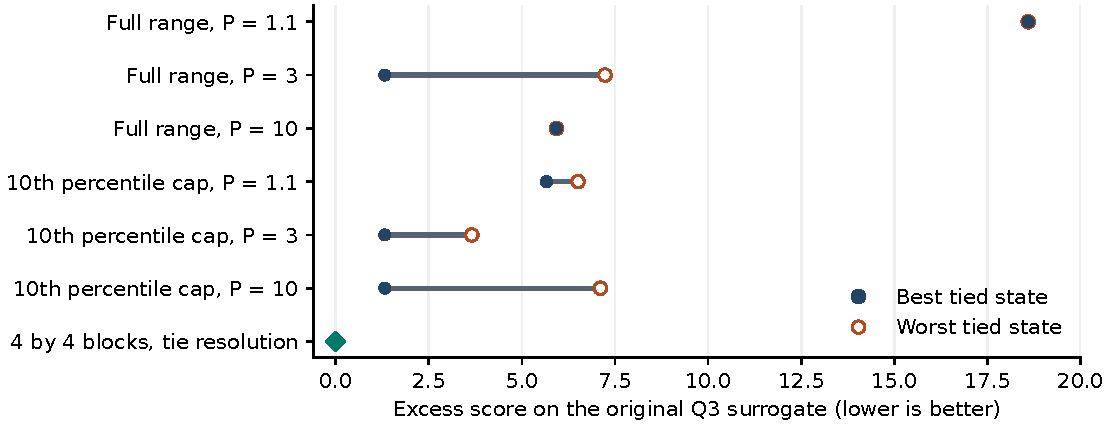
\includegraphics[width=.92\linewidth]{figures/precision.pdf}
\caption{Q3 original-score excess among legal states minimizing each quantized whole-grid energy. A segment spans tied outcomes. Coincident endpoints indicate identical excess. The diamond gives the verified result of the block method.}\label{fig:precision}
\end{figure}

\clearpage
\section{An eight-bit encoding with a checkable minimum}
All six whole-grid configurations in Figure~\ref{fig:precision} lose the minimum of the frozen mixture. For the full range and $P=1.1$, the winning legal pair costs an extra 18.5949 units of $\Vh$. A cap and $P=3$ reduce the best tied excess to 1.3175, still above zero. This audit checks only legal states. We now construct smaller blocks whose entire unconstrained state spaces can be checked.

Sort A and B alphabetically and partition each into thirteen consecutive groups of four. Each of the resulting 169 blocks $T$ covers 16 pairs. Let $M=\max_{ij\in T} C_{ij}$. For nonnegative costs use
\begin{equation}
 q_{ij}=\operatorname{round}(15C_{ij}/M),\quad
 q_{ij}\in\{0,\ldots,15\},\qquad P=16. \label{eq:bins}
\end{equation}
If $M=0$ set the whole block to zero. Use $q$ in Eq.~\eqref{eq:qubo}. A legal state has energy at most 15, whereas every illegal state costs at least 16. Rounding is monotone: the original block minimum is among the rounded minima. Retrieve the complete set of tied minima, read their original costs and keep the least. Comparing the 169 retained original costs recovers the global minimum. This proof depends on retrieving every ground state in a tied block. A sampler returning one arbitrary optimum has a weaker guarantee.

\subhead{Why the coefficients fit}
Write the upper-triangular QUBO with diagonal $-16$, within-group interactions $32$ and cross-group interactions $q_{ij}$, omitting the common constant 32. For eight bits $z$, set $s=2z-1$ and use one reference spin. With Kaiwu's $-s^\mathsf{T}Js$ convention, multiplying the returned symmetric matrix by eight gives integral couplings. Within-group entries are $-32$, cross-group entries are $-q_{ij}$. Each reference coupling is
\begin{equation}
 -\left(2(-16)+3(32)+\sum_{k=1}^4 q_{ik}\right)
 =-\left(64+\sum_{k=1}^4 q_{ik}\right),
\end{equation}
using the corresponding column sum on the B side. Its magnitude is at most 124. This is an a priori 8-bit bound for every block, independent of the absolute units of $\Vh$.

Kaiwu's \texttt{BruteForceOptimizer} solves the resulting nine-spin instances on the local CPU. We fix the gauge by multiplying every spin by the reference spin and deduplicate binary states. An independent pass checks all $2^8=256$ assignments in each block, including infeasible assignments. It verifies the affine energy relation, counts ground states, and compares every decoded optimum with the integer-cost table. Across both pools all 338 calls return complete sets of feasible ground states. Every retained block winner also matches the minimum of its original floating-point block.

\clearpage
\section{Selected compositions and computational cost}
\begin{table}[h]
\caption{Answers and membership checks. The two full pools are solved by Kaiwu. Direct scans of the two blind subsets give the restricted-pool comparison.}\label{tab:answers}
\centering\small\begin{tabular}{llrllrr}
\toprule Task & Pool (size) & ID & $(A,B,X)$ & Formula & $\Vh$ & Public $V$\\\midrule
Q2 & 07 (2,704)&13153& La, Ti, NO2 & LaTiO$_2$N & 6.924382 & hidden\\
Q3 & 08 (8,112)&8760& Sn, Ti, O3 & SnTiO$_3$ & 3.268113 & 0.001419\\\midrule
Q2 & 11 (529)&13153& La, Ti, NO2 & LaTiO$_2$N & 6.924382 & hidden\\
Q3 & 12 (1,587)&13153& La, Ti, NO2 & LaTiO$_2$N & 6.924382 & hidden\\\bottomrule
\end{tabular}
\end{table}
The winners in Table~\ref{tab:answers} use the same refitted model. The ordered triplets explain why the file's NO2 family is written as O$_2$N in the supplied formula. For Q2 and Q3, respectively, runner-up scores are 7.256664 and 3.904881. Enumeration gaps for the chosen records are zero. Their winning-block Ising energies under $-s^\mathsf{T}Js$ are $-702$ and $-724$. Constants and scales vary by block, so comparing those two energies would have no physical meaning. $\mathrm{SnTiO_3}$ belongs to file 02; its public value is an in-training observation after refitting. For a new DFT calculation in the blind pool, both objectives nominate $\mathrm{LaTiO_2N}$.

\begin{table}[h]
\caption{Wall-clock measurements on an AMD Ryzen 9 8945HX CPU. Fitting the three-component model is shared across both optimization problems.}\label{tab:cost}
\centering\small\begin{tabular}{lrr}
\toprule Stage & Q2 & Q3\\\midrule
Descriptors, shared (s) & \multicolumn{2}{c}{\DescFull}\\
Refit on 15,225 rows, shared (s) & \multicolumn{2}{c}{\FitFull}\\
Score 8,112 rows, shared (s) & \multicolumn{2}{c}{\ScoreFull}\\
Subset, index and reduce pool (s) & \PoolTwo & \PoolThree\\
Construct and convert 169 blocks (s) & \EncodeTwo & \EncodeThree\\
169 Kaiwu CPU solves (s) & \SolveTwo & \SolveThree\\
Decode, resolve ties, verify (s) & \CheckTwo & \CheckThree\\
Direct array minimum, median ($\mu$s) & \ScanTwo & \ScanThree\\
Blocks with ties / 169 & \TiedTwo & \TiedThree\\
Original costs compared within tied or unique minima & \FinalistsTwo & \FinalistsThree\\
Observed integer coupling range & $[\CoeffLowTwo,0]$ & $[\CoeffLowThree,0]$\\\bottomrule
\end{tabular}
\end{table}
The direct scan uses the same in-memory predictions and times 1,001 repetitions of one array minimum. The larger QUBO times include the checks itemized above; disk I/O and manuscript generation lie outside these timings. For Q1 alone, descriptors, training and scoring the hidden set took \DescOne, \FitOne\ and \ScoreOne\ seconds. These are local wall times under the observed machine load. Device programming, queueing, sampling, energy consumption and hardware success rates remain unmeasured.

\clearpage
\section{Interpretation and limits}
Two kinds of error matter to a one-composition decision. For any returned candidate $u$ and a true minimizer $u^*$ in the same pool, adding and subtracting predicted scores yields
\begin{equation}
 V(u)-V(u^*)\ \leq\
 2\max_{z}|V(z)-\Vh(z)|+
 \underbrace{\Vh(u)-\min_z\Vh(z)}_{\text{optimization gap}} .
 \label{eq:regret}
\end{equation}
The maximum is taken over that pool. The second term is exactly zero for our full-pool results. The first term cannot be estimated uniformly on hidden compositions from a mean validation error. For example, even selecting the exact minimum of the primary surrogate on Q3 validation incurs physical regret 11.45225. Two models that agree on average can still disagree where the minimum lies.

The metallic lower bound exploits an empirical identity in this particular dataset and can transfer only where the energy conventions remain valid. A single material outside the assumed branch may give a confident wrong choice. In the unseen-pair folds the mixture finds 23 of 50 three-family near-targets at 50 checks per fold, compared with 14 for direct regression. Their median single-choice regrets are 13.521 and 11.569, respectively. These measurements support shortlist enrichment more strongly than a one-shot prediction. A physical calculation for the blind winner would provide information unavailable from any additional optimization of the frozen scores.

The eight-bit construction controls a different risk. Small, exactly solved blocks allow the original-score minimum to survive ties, while increasing classical work. A large hardware instance has programming and readout costs and may miss tied ground states. Benchmarking a device would require observed success probabilities and end-to-end timings on comparable inputs \cite{speed}. In the present search, every composition is scored before optimization, and a direct scan already attains the same minimum in microseconds. The experiment establishes finite-precision correctness on the local Kaiwu backend. The performance and physical outcome of an SPQC run remain open.

For the requested full pools the single choices are therefore $\mathrm{LaTiO_2N}$ for Q2 and $\mathrm{SnTiO_3}$ for Q3. If the next action is to assay an unlabeled composition, the common blind-pool choice is $\mathrm{LaTiO_2N}$. Its predicted score of 6.924382 leaves its physical status unresolved.

